   
\chapter*{Notation}
\addcontentsline{toc}{fmbm}{Notation}
\addtocontents{toc}{\protect\enlargethispage{1\baselineskip}}

\marginnote{We will use notes inside boxes to bring attention to important concepts, or to add additional comments without breaking the flow of the main text.}
This book deals with many different fields and each has its own notation. We will stick to the following conventions throughout most of this book, and indicate when we deviate from these rules. To define the conventions we give examples of usage, from which you can infer the pattern.

\subsection*{General Notation}
\begin{itemize}
\item Scalar: $x$, $y$, $z$.
\item Vector: $\mathbf{x}, \mathbf{y}, \mathbf{z}$. We use bold letters to represent vectors, matrices, and tensors.
\item Index of a vector: $x_i$, $x_j$, $y_i$, or $x[i]$, $x[j]$, $y[i]$.
\item Matrix: $\mathbf{X}$, $\mathbf{Y}$, $\mathbf{Z}$. We use bold letters to represent vectors, matrices, and tensors.
\item Index of a matrix: $X_{ij}$, $Y_{jk}$, $Z_{ii}$, or $X[i,j]$, $Y[j,k]$, $Z[i,i]$.
\item For an indexed matrix $X_{ij}$ or $X[i,j]$, $i$ indexes rows and $j$ indexes columns. We use non-bold font because $X_{ij}$ and $X[i,j]$ are scalars.
\item Slice of a matrix: $\mathbf{X}_i$ or $\mathbf{X}[i,:]$; $\mathbf{X}[:,j]$. Here is one example, using zero-based indexing:
\begin{align*}
\mathbf{X} = 
\begin{bmatrix}
    1 & 2 \\
    3 & 4 \\
    5 & 6
\end{bmatrix}
&&
\mathbf{X}[2,:] = 
\begin{bmatrix}
    5 & 6
\end{bmatrix}
\end{align*}
\item Tensor (i.e., multidimensional arrays): Typically, we will use lowercase bold variables to represent tensors, for example, $\mathbf{x}$. This is because tensors can have any number of dimensions (they can be one-dimensional, two-dimensional, three-dimensional, and so on). Furthermore, we will often define operators that are agnostic to the dimensionality of the tensor (they apply to $N$-dimensional arrays, for any $N$). However, in some sections, we use uppercase to make a distinction between tensors of different shapes, and we will specify when this is the case. 
\marginnote{
A 3D tensor that could represent a $C \times H \times W$ color image: 
\\[6pt]
\centerline{
\includegraphics[width=.25\linewidth]{figures/neural_nets/3D_tensor_example.eps}
}
}[-0.05in]
\item Index or slice of a tensor: $x[c,i,j,k]$, $\mathbf{x}[:,:,k]$; if $\mathbf{x}$ is a multidimensional tensor and we wish to slice by the first dimension, we may use $\mathbf{x}_t$ or $\mathbf{x}[t]$ or $\mathbf{x}[t,:]$, all of which have the same meaning.
%\item When the dimensionality of a variable is arbitrary (can take on different values in different settings) we will consider it a tensor and use the tensor notation.
\item A set of $N$ datapoints: $\{x^{(i)}\}_{i=1}^N$, $\{\mathbf{x}^{(i)}\}_{i=1}^N$, $\{\mathbf{X}^{(i)}\}_{i=1}^N$
%\item $\mathbf{A} = [\mathbf{x},\mathbf{y},\mathbf{z}]$ concatenates column vectors $\mathbf{x},\mathbf{y},\mathbf{z}$ as columns of matrix $A$. $\mathbf{A} = [\mathbf{x}^\transpose,\mathbf{y}^\transpose,\mathbf{z}^\transpose]$ concatenates these vectors as rows of $\mathbf{A}$. 
\item Dot product: $\mathbf{x}^\transpose\mathbf{y}$
\item Matrix product: $\mathbf{A}\mathbf{B}$
\item Hadamard product (i.e., element-wise product): $\mathbf{x} \hadamard \mathbf{y}$, $\mathbf{A} \hadamard \mathbf{B}$
\item Product of two scalars: $ab$ or $a*b$ 
\end{itemize}
\marginnote{In the geometry chapters, and in some other chapters, the variables $x$, $y$, $z$ will denote location and will have a special treatment.}[-0.2in]


\subsection*{Signal Processing}
\begin{itemize}
\item Discrete signals (and images) are vectors $\mathbf{x}, \mathbf{y}, \mathbf{z}$.
\item When indexing a discrete signal we will use brackets: $x \left[ n\right]$, where $n$ is a discrete index.
\item Continuous signals are denoted $x (t)$, where $t$ is a continuous variable.
\item Convolution operator: $\circ$
\item Cross-correlation operator: $\star$
\item Discrete Fourier transforms: $X \left[ u\right]$, where $u$ is a discrete frequency index.
\end{itemize}

\subsection*{Images}

Images are a very special signal and, whenever is convenient, we will use the following notation:
\marginnote{We will use the letter $\img$, from $\img$ight, when the signal is an image. We use this letter because it is very distinct from all the other notation. But sometimes we will use other notation if it is more convenient.}
\begin{itemize}
\item Image as a discrete 2D signal: $\img \left[ n,m \right]$ where $n$ indexes columns and $m$ indexes rows. The origin, $n=m=0$, corresponds to the bottom-left side of the image unless we specify a different convention. An image has a size $N \times M$, $N$ columns and $M$ rows. 
\item Image as a matrix: $\boldimg$ of size $M \times N$, $M$ rows and $N$ columns, which can be indexed as $\img_{ij}$.
\item The Fourier transform on an image: $\capitalimg \left[ u,v\right]$, where $u$ and $v$ are spatial frequencies.
\end{itemize}
Note that the way matrices and images are indexed is transposed. However, we will rarely represent images as arrays. If we do, we will use the general notation and the images will be just generic signals, $\mathbf{x}, \mathbf{y}, \mathbf{z}$. 

\subsection*{Machine Learning}
\begin{itemize}
    \item Total loss function / cost function / objective function: $J$
    \item Per-datapoint loss function: $\mathcal{L}$
    \item Generic learnable parameters: $\theta$
\end{itemize}


\subsection*{Neural Networks}
\begin{itemize}
\item \textit{Parameters}: $\theta$. These include weights, $\mathbf{W}$, and biases, $\mathbf{b}$, as well as any other learnable parameters of a network.
\item \textit{Data}: $\mathbf{x}$. Data can refer to inputs to the network, activations on hidden layers, outputs from the network, and so on. Any representation of the signal being processed is considered to be data. Sometimes we will wish to distinguish between the raw inputs, hidden units, and outputs to a network, in which case we will use $\mathbf{x}$, $\mathbf{h}$, and $\mathbf{y}$ respectively. When we need to to distinguish between pre-activation hidden units and postactivation, we will use $\mathbf{z}$ for pre-activation and $\mathbf{h}$ for postactivation.
\marginnote{
%Neural net:
%~\\
%\begin{figure}
%\centerline{
%\noindent\hspace{0.05\linewidth}
%\begin{minipage}%{1\linewidth}
\centerline{
\begin{tikzpicture}[>=spaced latex]
\draw [thick, fill=white] (0,-0.4) circle [radius=0.3] node {$x_2$};
\draw [thick, fill=white] (0,0.4) circle [radius=0.3] node {$x_1$};
\draw [thick] [nn_edge] (0.3,-0.4) -- (1.0,-0.05) node[midway,below] {$w_2$};
\draw [thick] [nn_edge] (0.3,0.4) -- (1.0,0.05) node[midway,above] {$w_1$};
\draw [thick, fill=gray_neuron] (1.3,0) circle [radius=0.3] node {$z$};
\draw [thick] [nn_edge] (1.6,0) -- (2.3,0);
\draw [thick, fill=white] (2.6,0) circle [radius=0.3] node {$y$};
\end{tikzpicture}
%\end{minipage}
%}
%\end{figure}
}
}

\item When describing batches of tensors (as is commonly encountered in code), you may encounter $x_l[b,c,n,m]$ to represent an activation on layer $l$ of some network, with $b$ indexing batch element, $n$ and $m$ as spatial coordinates, and $c$ indexing channels.
\item Neuron values on layer $l$ of a deep net: $\mathbf{x}_{l}$
\item $x_{l}[n]$ refers to the $n$-th neuron on layer $l$. For neural networks with spatial feature maps (such as convolutional neural networks), each layer is an array of neurons, and we will use notation such as $x_{l}[n,m]$ to index the neuron at location $n,m$.
%\item For a network with spatial feature maps (e.g., a convolutional neural network), $x_{l}[c,i,j]$ refers to the $cij$-th neuron on layer $l$, where $i$ and $j$ index spatial position in a feature map, and $c$ indexes the channel.
\item The layer $l$ neural representation of the $i$-th datapoint in a dataset is written as $\mathbf{x}^{(i)}_{l}$.
\item We will also use $\xin$ and $\xout$ when we are describing a particular layer or module in a neural net and wish to speak of its inputs and outputs without having to keep track of layer indices.
\item For signals with multiple channels, including neural network feature maps, the first dimension of the tensor indexes over channel. For example, in $\mathbf{x} \in \mathbb{R}^{C \times N \times M \times \ldots}$, where $C$ is the number of channels of the signal.
\item For transformers, we deviate from the previous point slightly, in order to match standard notation: a set of tokens (which will be defined in the transformers chapter) is represented by a $[N \times d]$ matrix, where $d$ is the token dimensionality.
\end{itemize}


\subsection*{Probabilities}

We will sometimes not distinguish between random variables and realizations of those variables; which we mean should be clear from context. When it is important to make a distinction, we will use nonbold capital letters to refer to random variables and lowercase to refer to realizations.

Suppose $X, Y$ are discrete random variables and $\mathbf{x}, \mathbf{y}$ are realizations of those variables. $X$ and $Y$ may take on values in the sets $\mathcal{X}$ and $\mathcal{Y}$, respectively.
\begin{itemize}
    \item $a = p(X = \mathbf{x} \given \ldots)$ is the probability of the realization $X = \mathbf{x}$, possibly conditioned on some observations ($a$ is a scalar).
    \item $f = p(X \given \ldots)$ is the probability distribution over $X$, possibly conditioned on some observations ($f$ is a function: $f: \mathcal{X} \rightarrow \mathbb{R}$). If $\mathcal{X}$ is discrete, $f$ is the \emph{probability mass function}. If $\mathcal{X}$ is continuous, $f$ is the \emph{probability density function}.
    %\item $a = p(X = x | \overset{R}{y} = y)$ is the probability of the realization $\overset{R}{x}=x$ given $\overset{R}{y}=y$ ($a$ is a scalar).
    %\item $f = p(\overset{R}{x} | \overset{R}{y} = y)$ is the probability distribution over $\overset{R}{x}$ given $\overset{R}{y}=y$ ($f: \mathcal{X} \rightarrow \mathbb{R}$).
    %\item $f = p(\overset{R}{x} = x | \overset{R}{y})$ is a function with the property $f(y) = p(\overset{R}{x} = x | \overset{R}{y} = y)$ ($f: \mathcal{Y} \rightarrow \mathbb{R}$).
    %\item $p(\overset{R}{x} | \overset{R}{y})$ is the conditional probability distribution of $\overset{R}{x}$ given $\overset{R}{y}$ ($f: \mathcal{X} \times \mathcal{Y} \rightarrow \mathbb{R}$).
    %\item $p(x)$ is shorthand for $p(\overset{R}{x} = x)$.
    %\item $p(x|y)$ is shorthand for $p(\overset{R}{x} = x | \overset{R}{y} = y)$.
    %\item Suppose we have defined a named distribution, e.g., $p_{\theta}$; then referring to $p_{\theta}$ on its own is shorthand for $p(\overset{R}{x})$. This often comes up in expressions like $x \sim p_{\theta}$, which refers to $\overset{R}{x}$ as being distributed as $p_{\theta}(\overset{R}{x})$.
    %\item $p(\overset{R}{x} | y)$ is shorthand for $p(\overset{R}{x} | \overset{R}{y} = y)$
    \item $p(\mathbf{x} \given \ldots)$ is shorthand for $p(X = \mathbf{x} \given \ldots)$.
    %\item $p(\ldots | y)$ is shorthand for $p(\ldots | \overset{R}{y} = y)$.
    and so forth, following these patterns.
    \item Suppose we have defined a named distribution, for example, $p_{\theta}$, for some random variable $X$; then referring to $p_{\theta}$ on its own is shorthand for $p_{\theta}(X)$.
    \item We will write $Z \sim p$ to indicate a random variable whose distribution is $p$, and we will write $z \sim p$ to indicate a sampled realization of such a variable.
\end{itemize}
For continuous random variables, all the above notations hold except that they refer to probability densities and probability density functions rather than probabilities and probability distributions. We will sometimes also use the term ``probability distribution'' for continuous random variables, and in those cases it should be understood that we are referring to a probability density function.


\subsection*{Matrix Calculus Conventions}
\label{appendix:matrix_calc:notational_conventions}

In this book, we adopt the following conventions for matrix calculus. These conventions make the equations simpler, and that also means simpler implementations when it comes to actually writing these equations in code. Everything in this section is just definitions. There is no right or wrong to it. We could have used other conventions but we will see that these are useful ones.

Vectors are represented as column vectors with shape $[N \times 1]$:
\begin{align}
    \mathbf{x} = 
    \begin{bmatrix}
    x_1  \\
    x_2  \\
    \vdots \\
    x_N \\
    \end{bmatrix}
\end{align}
If $y$ is a scalar and $\mathbf{x}$ is an $N$-dimensional vector, then the gradient $\frac{\partial y}{\partial \mathbf{x}}$ is a row vector of shape  $[1 \times N]$:
\begin{align}
    \frac{\partial y}{\partial \mathbf{x}} =  
\begin{bmatrix}
    \frac{\partial y}{\partial x_1} & \frac{\partial y}{\partial x_2} & \cdots & \frac{\partial y}{\partial x_N} \label{backprop:scalar_vector_deriv}
\end{bmatrix}
\end{align}
If $\mathbf{y}$ is an $M$-dimensional vector and $\mathbf{x}$ is a $N$-dimensional vector then the gradient (also called the Jacobian in this case) is shaped as $[M \times N]$:
\begin{align}
\frac{\partial \mathbf{y}}{\partial \mathbf{x}} =  
\begin{bmatrix}
    \frac{\partial y_1}{\partial x_1} & \frac{\partial y_1}{\partial x_2} & \cdots & \frac{\partial y_1}{\partial x_N} \\
    \vdots & \vdots & \vdots & \vdots \\
    \frac{\partial y_M}{\partial x_1} & \frac{\partial y_M}{\partial x_2} & \cdots & \frac{\partial y_M}{\partial x_N}
\end{bmatrix}
\end{align}


Finally, if $\mathbf{W}$ is an $[N \times M]$ dimensional matrix, and $\mathcal{L}$ is a scalar, then the gradient $\frac{\partial \mathcal{L}}{\mathbf{W}}$ is represented as an $[M \times N]$ dimensional matrix (note that the dimensions are transposed from what you might have expected; this makes the math simpler later):
\begin{align}
    \frac{\partial \mathcal{L}}{\partial \mathbf{W}} &= 
        \begin{bmatrix}
            \frac{\partial \mathcal{L}}{\partial \mathbf{W}_{11}} & \ldots & \frac{\partial \mathcal{L}}{\partial \mathbf{W}_{N1}} \\
            \vdots & \ddots & \vdots \\
            \frac{\partial \mathcal{L}}{\partial \mathbf{W}_{1M}} & \ldots & \frac{\partial \mathcal{L}}{\partial \mathbf{W}_{NM}} \\
        \end{bmatrix} \label{backprop:scalar_matrix_deriv}
\end{align}
\marginnote{
We will often draw matrices and vectors to help visualize the operations. For example, if $N=3$ and $M=4$:\\[2pt]
\centerline{
\begin{tikzpicture}
\draw[step=0.25cm,draw=black,fill=param_color_dark] (1.5,0) grid (2.5,-0.75) rectangle (1.5,0); \node at (2.0,0.25) {$\mathbf{W}$};
\end{tikzpicture}}
then, the gradient will have the form:\\[2pt]
\centerline{
\begin{tikzpicture}
\draw[step=0.25cm,draw=black,fill=comp_graph_param_grad_bcolor] (0,0) grid (0.75,-1.0) rectangle (0,0); \node at (0.375,0.3) {$\frac{\partial \mathcal{L}}{\partial \mathbf{W}}$};
\end{tikzpicture}}
}[-.9in]

\subsection*{Conventions That Will Not Be Strictly Observed}
\begin{itemize}
\item We will often use $\mathbf{x}$ as the input to a function, and $\mathbf{y}$ as the output.
\item $f$, $g$, and $h$ are typically functions. The corresponding function spaces are $\mathcal{F}$, $\mathcal{G}$, $\mathcal{H}$.
\item Basis functions are $\phi$ and $\psi$.
\end{itemize}

\subsection*{Miscellaneous}
\begin{itemize}
\item The word ``dimension'' has two usages in the computational sciences. The first usage is as a coordinate in a multivariate data structure, for example, ``the $i$-th dimension of a vector'' or ``a 128-dimensional feature space.'' The second usage is as the shape of a multidimensional array, as in ``a 4D tensor.'' We will use both these meanings in this book and we hope the usage will be clear from context.
\end{itemize}

